\documentclass[11pt, a4paper]{article}
\usepackage[english]{babel}
\usepackage{hyperref}
\usepackage{graphicx}
\usepackage{amsmath}
\usepackage{amssymb}
\usepackage{tabularx}
% LaTeX settings for MATLAB code listings
% based on Ted Pavlic's settings in http://links.tedpavlic.com/ascii/homework_new_tex.ascii
\usepackage{listings}
\usepackage[usenames,dvipsnames]{color}

% This is the color used for MATLAB comments below
\definecolor{MyDarkGreen}{rgb}{0.0,0.4,0.0}

% For faster processing, load Matlab syntax for listings
\lstloadlanguages{Matlab}%
\lstset{language=Matlab,                        % Use MATLAB
    	breakindent=40pt, 
   		breaklines,
        frame=single,                           % Single frame around code
        basicstyle=\small\ttfamily,             % Use small true type font
%		basicstyle=\footnotesize,
        keywordstyle=[1]\color{Blue}\bfseries,  % MATLAB functions bold and blue
        keywordstyle=[2]\color{Purple},         % MATLAB function arguments purple
        keywordstyle=[3]\color{Blue}\underbar,  % User functions underlined and blue
        identifierstyle=,                       % Nothing special about identifiers
                                                % Comments small dark green courier
        commentstyle=\usefont{T1}{pcr}{m}{sl}\color{MyDarkGreen}\small,
        stringstyle=\color{Purple},             % Strings are purple
        showstringspaces=false,                 % Don't put marks in string spaces
        tabsize=4,                              % 5 spaces per tab
        %
        %%% Put standard MATLAB functions not included in the default
        %%% language here
        morekeywords={xlim,ylim,var,alpha,factorial,poissrnd,normpdf,normcdf,specifyCoefficients},
        %
        %%% Put MATLAB function parameters here
        morekeywords=[2]{on, off, interp},
        %
        %%% Put user defined functions here
        morekeywords=[3]{FindESS, homework_example},
        %
        morecomment=[l][\color{Blue}]{...},     % Line continuation (...) like blue comment
        numbers=left,                           % Line numbers on left
        firstnumber=1,                          % Line numbers start with line 1
        numberstyle=\tiny\color{Blue},          % Line numbers are blue
        stepnumber=1                            % Line numbers go in steps of 5
        }

% Includes a MATLAB script.
% The first parameter is the label, which also is the name of the script
%   without the .m.
% The second parameter is the optional caption.
\newcommand{\matlabscript}[2]
  {\begin{itemize}\item[]\lstinputlisting[caption=#2,label=#1]{#1.m}\end{itemize}}

\title{PDE Toolbox example}
\author{Gilbert Fran\c cois Duivesteijn}

\begin{document}
\maketitle

\begin{figure}
  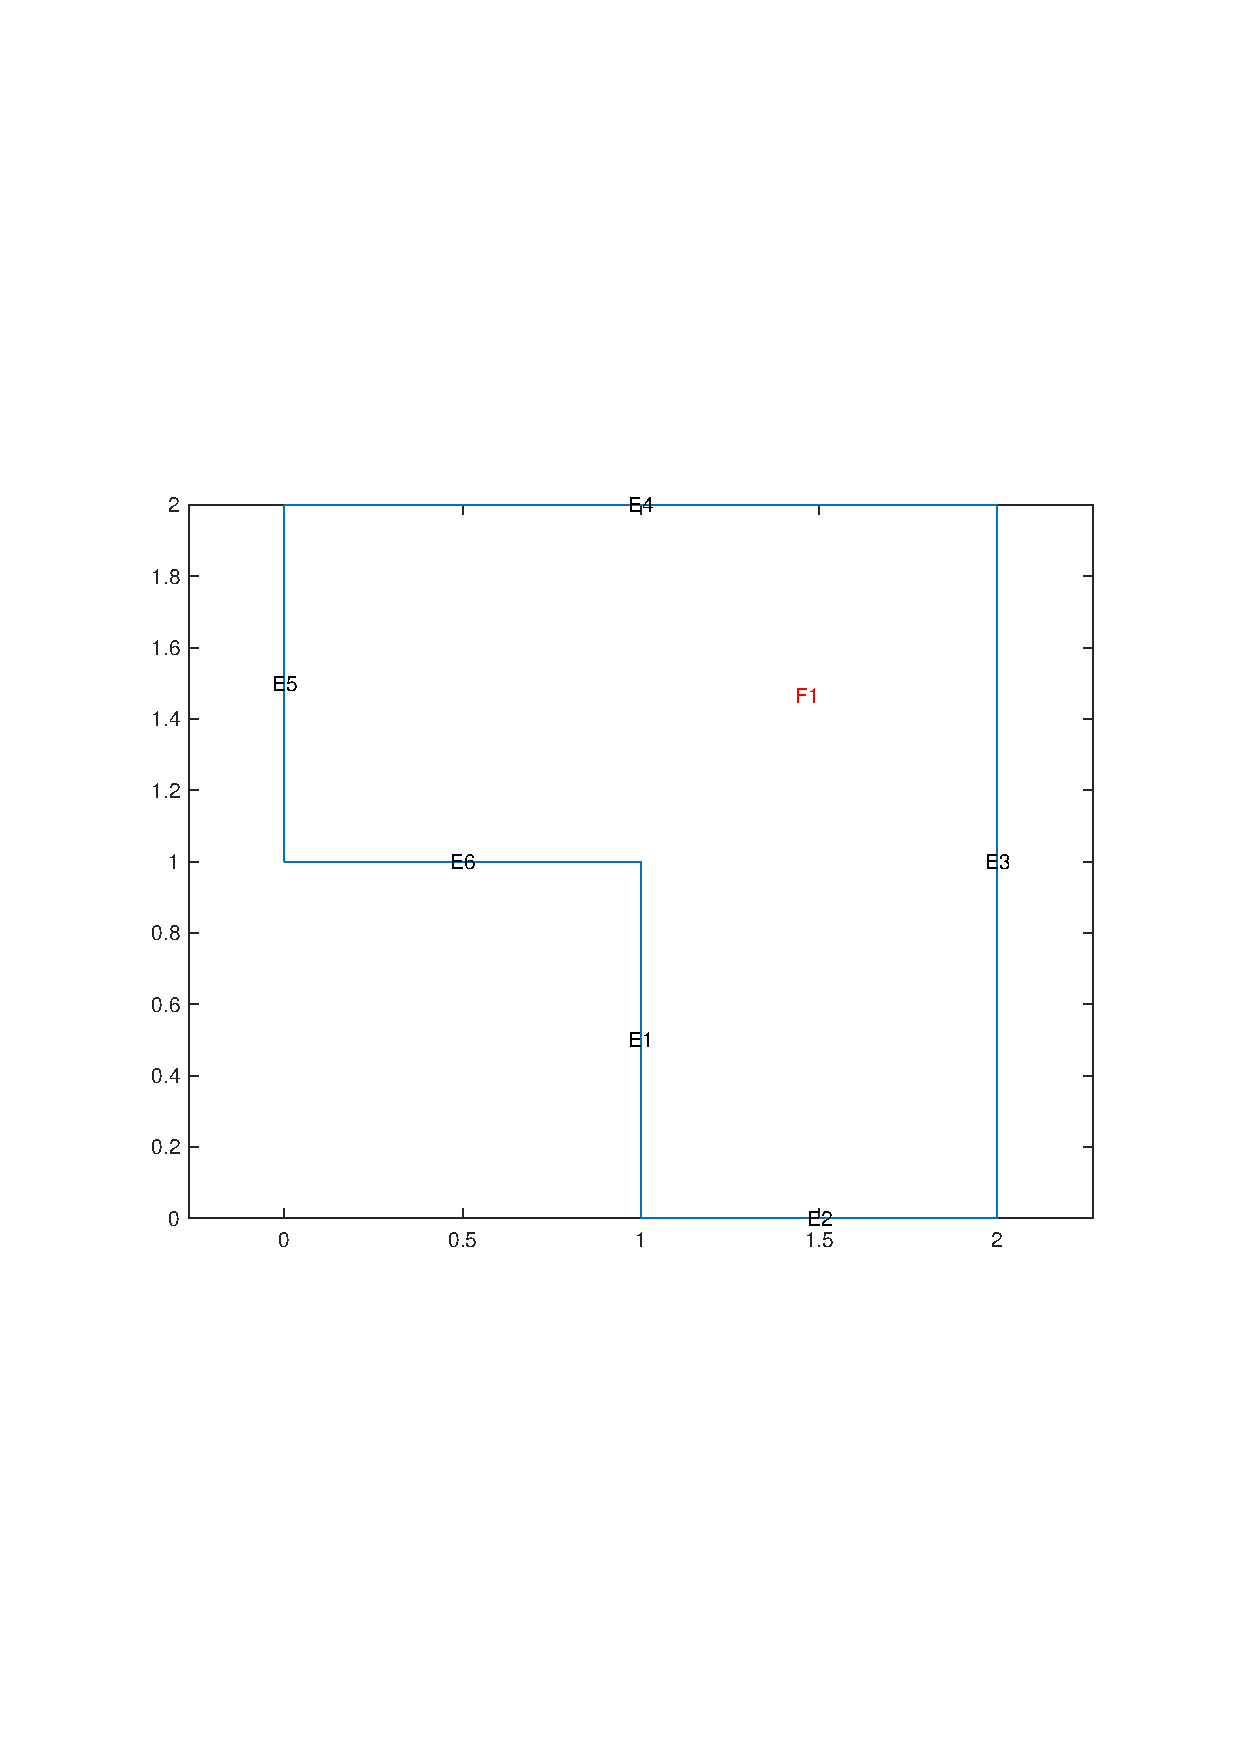
\includegraphics[width=0.49\textwidth]{assets/domain.pdf}
  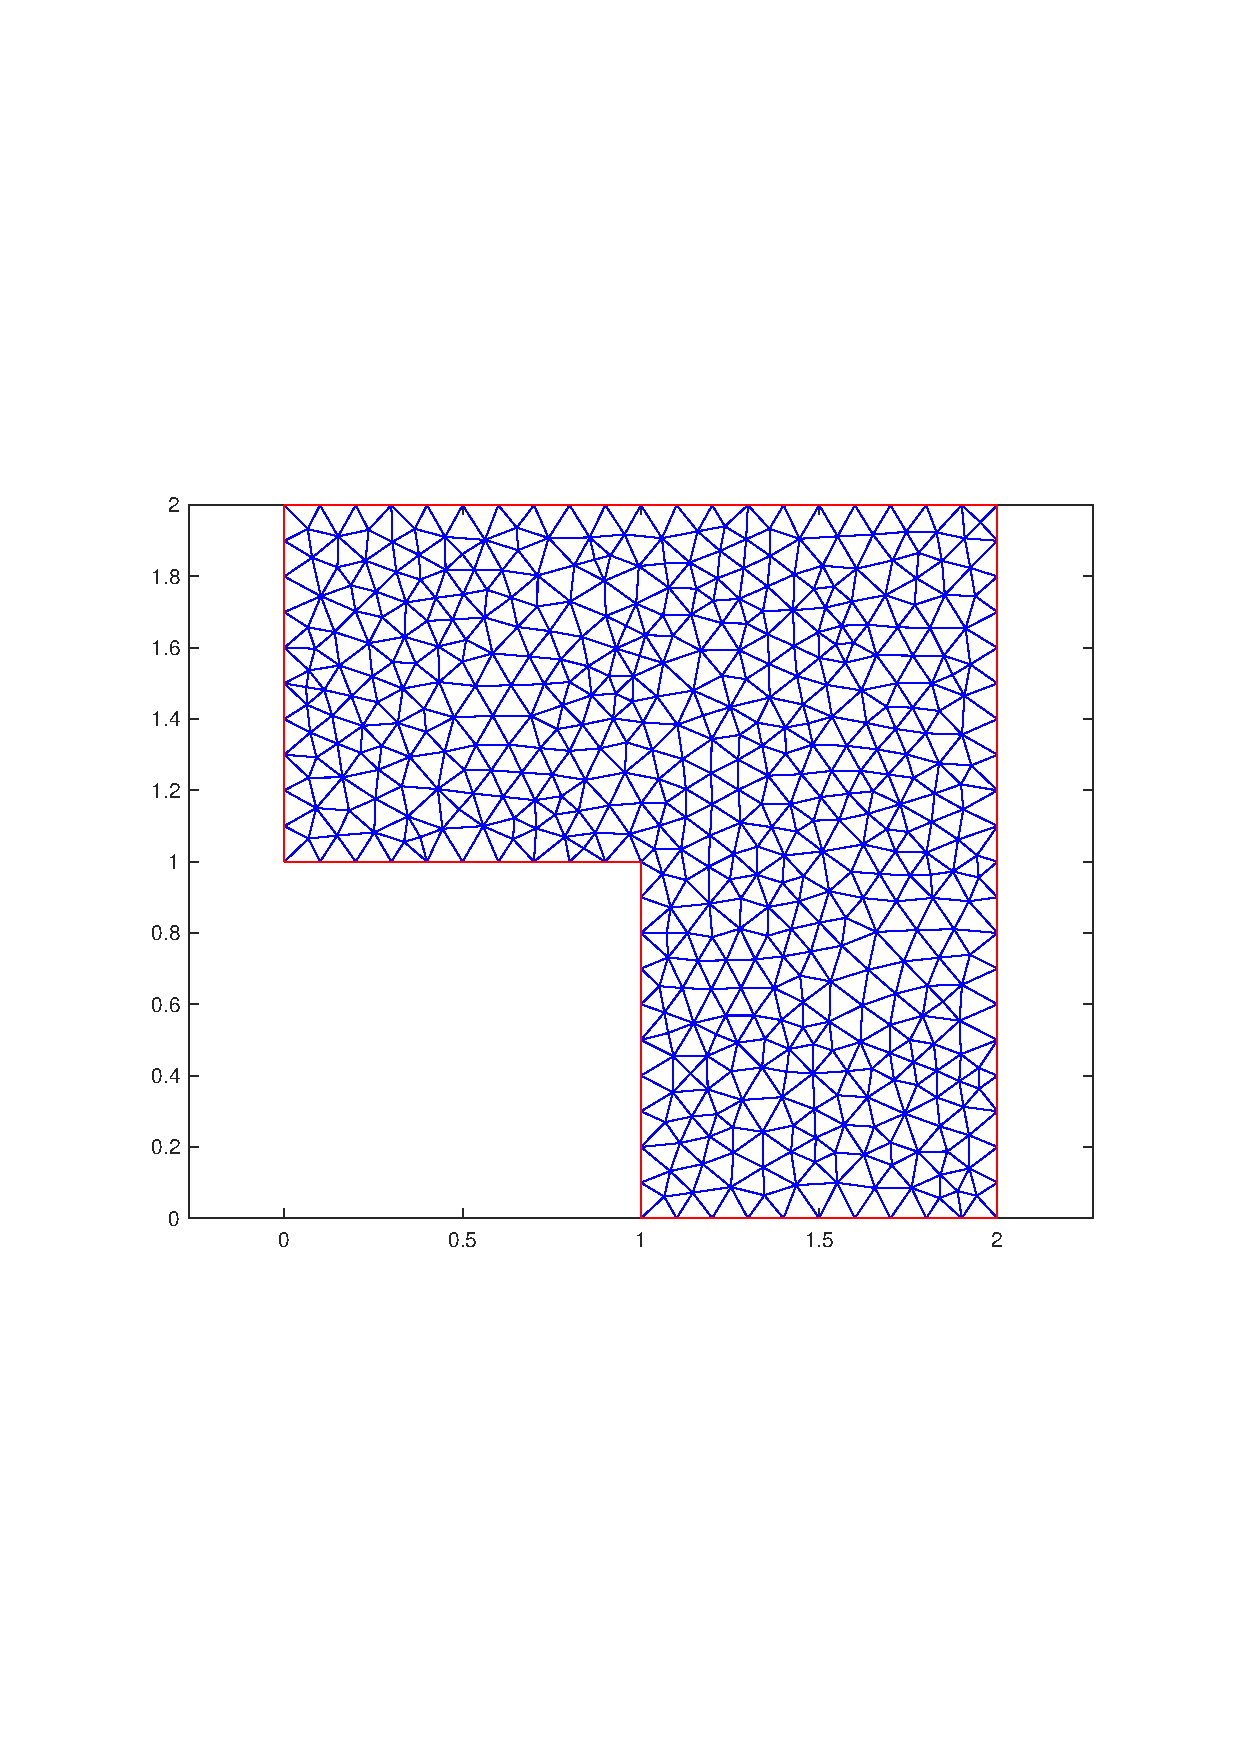
\includegraphics[width=0.49\textwidth]{assets/grid.pdf}
  \caption{Computational domain with edge and face labels (left). Unstructured grid (right).}\label{fig:domain}
\end{figure}

This is a simple example, showing how to use the Matlab PDE toolbox\footnote{\href{https://www.mathworks.com/help/releases/R2017a/pde/index.html}{PDE Toolbox documentation}}. The recommended workflow is
\begin{itemize}
	\item Create PDE\footnote{\href{https://www.mathworks.com/help/releases/R2017a/pde/ug/createpde.html}{createpde}}
	\item Define geometry\footnote{\href{https://www.mathworks.com/help/releases/R2017a/pde/ug/decsg.html}{decsg}}
	\item Apply boundary conditions\footnote{\href{https://www.mathworks.com/help/releases/R2017a/pde/ug/applyboundarycondition.html}{applyboundarycondition}}
	\item Specify coefficients\footnote{\href{https://www.mathworks.com/help/releases/R2017a/pde/ug/specifycoefficients.html}{specifycoefficients}}
	\item Set initial conditions\footnote{\href{https://www.mathworks.com/help/releases/R2017a/pde/ug/setinitialconditions.html}{setinitialconditions}}
	\item Generate mesh\footnote{\href{https://www.mathworks.com/help/releases/R2017a/pde/ug/generatemesh.html}{generatemesh}}
	\item Solve the PDE\footnote{\href{https://www.mathworks.com/help/releases/R2017a/pde/ug/solvepde.html}{solvepde}}
\end{itemize}


Let's analyse the L-shaped domain (figure \ref{fig:domain}) and solve the molecular diffusion equation 
\begin{align}
\frac{\partial u}{\partial t} &= D \nabla^2 u \\ \label{eq:pde}
\end{align}
with boundary conditions
\begin{align}
\frac{\partial u}{\partial \textbf{n}} &= 0  \qquad \textrm{on} \quad [E_2, E_3, E_4, E_5] \label{eq:bc1}\\
u &= 0 \qquad \textrm{on} \quad [E_1, E_6] \label{eq:bc2}\\
\end{align}
and initial condition
\begin{align}
u(t=0) &= e^{-16(x-\frac{1}{2})^2-16(y-\frac{1}{2})^2}	\qquad \textrm{on} \quad F_1 \label{eq:init}
\end{align}


Matlab has a generic PDE formula that you can tune to your problem by setting the coefficients. The solvepde function models the equation:
\begin{align}
m\frac{\partial^2 u}{\partial t^2} + d\frac{\partial u}{\partial t} - \nabla \cdot (c\nabla u) + au &= f \label{eq:pde_ref}	
\end{align}
The coefficients to set are $m$, $d$, $c$, $a$ and $f$. To define (\ref{eq:pde}), we set $m=0$, $d=1$, $c=D$, $a=0$ and $f=0$.

\begin{lstlisting}[language=Matlab]
%% Specify the PDE model

specifyCoefficients(    ...
    model,              ...
    'm', 0,             ...
    'd', 1,             ...
    'c', 0.05,          ...
    'a', 0,             ...
    'f', 0              ...
);	
\end{lstlisting}

Note that the Dirichlet and Neumann boundary conditions are defined in a generic way, that can be tailored to the specific use case by setting the coefficients. The Dirichlet boundary condition implies that the solution u on a particular edge or face satisfies the equation
\begin{align}
	hu = r
\end{align}
where $h$ and $r$ are functions defined on $\partial \Omega$. Generalized Neumann boundary conditions imply that the solution u on the edge or face satisfies the equation
\begin{align}
\textbf{n}\cdot (c\nabla u) + qu = g	
\end{align}
The coefficient $c$ is the same as the coefficient of the second order differential operator in the generic partial differential equation (\ref{eq:pde_ref}). When specifying the boundary conditions, we give the type (e.g. `neumann' or `dirichlet'), the list of edges, as seen in figure \ref{fig:domain} and the coefficients. The boundary conditions from (\ref{eq:bc1}) and (\ref{eq:bc2}) are:

\begin{lstlisting}[language=Matlab]
%% Boundary conditions

applyBoundaryCondition(model,           ...
    'neumann', 							...
    'edge', [2, 3, 4, 5],  				...
    'g', 0,                             ...
    'q', 0                              ...
);

applyBoundaryCondition(model,           ...
    'dirichlet', 						...
    'edge', [1, 6],        				...
    'u', 0);
	
\end{lstlisting}

Let's set the initial condition from equation (\ref{eq:init}) by creating a function at the end of the script and reference the function pointer in the function setInitialConditions.

\begin{lstlisting}[language=Matlab]
%% Initial conditions.

setInitialConditions(model, @fn_u0);

%% Function declarations

function u0 = fn_u0(location)
    u0(1,:) = exp(-16*(location.x-1.5).^2 ...
                  -16*(location.y-1.5).^2);
end
\end{lstlisting}

Generate the mesh, solve the PDE and get the results from the result object:
\begin{lstlisting}[language=Matlab]
%% Generate mesh.
generateMesh(model, 'Hmax', 0.1);

%% Time domain
t = 0:0.01:10;

%% Solve the PDE
result = solvepde(model, t);
u = result.NodalSolution;
\end{lstlisting}

\begin{figure}
  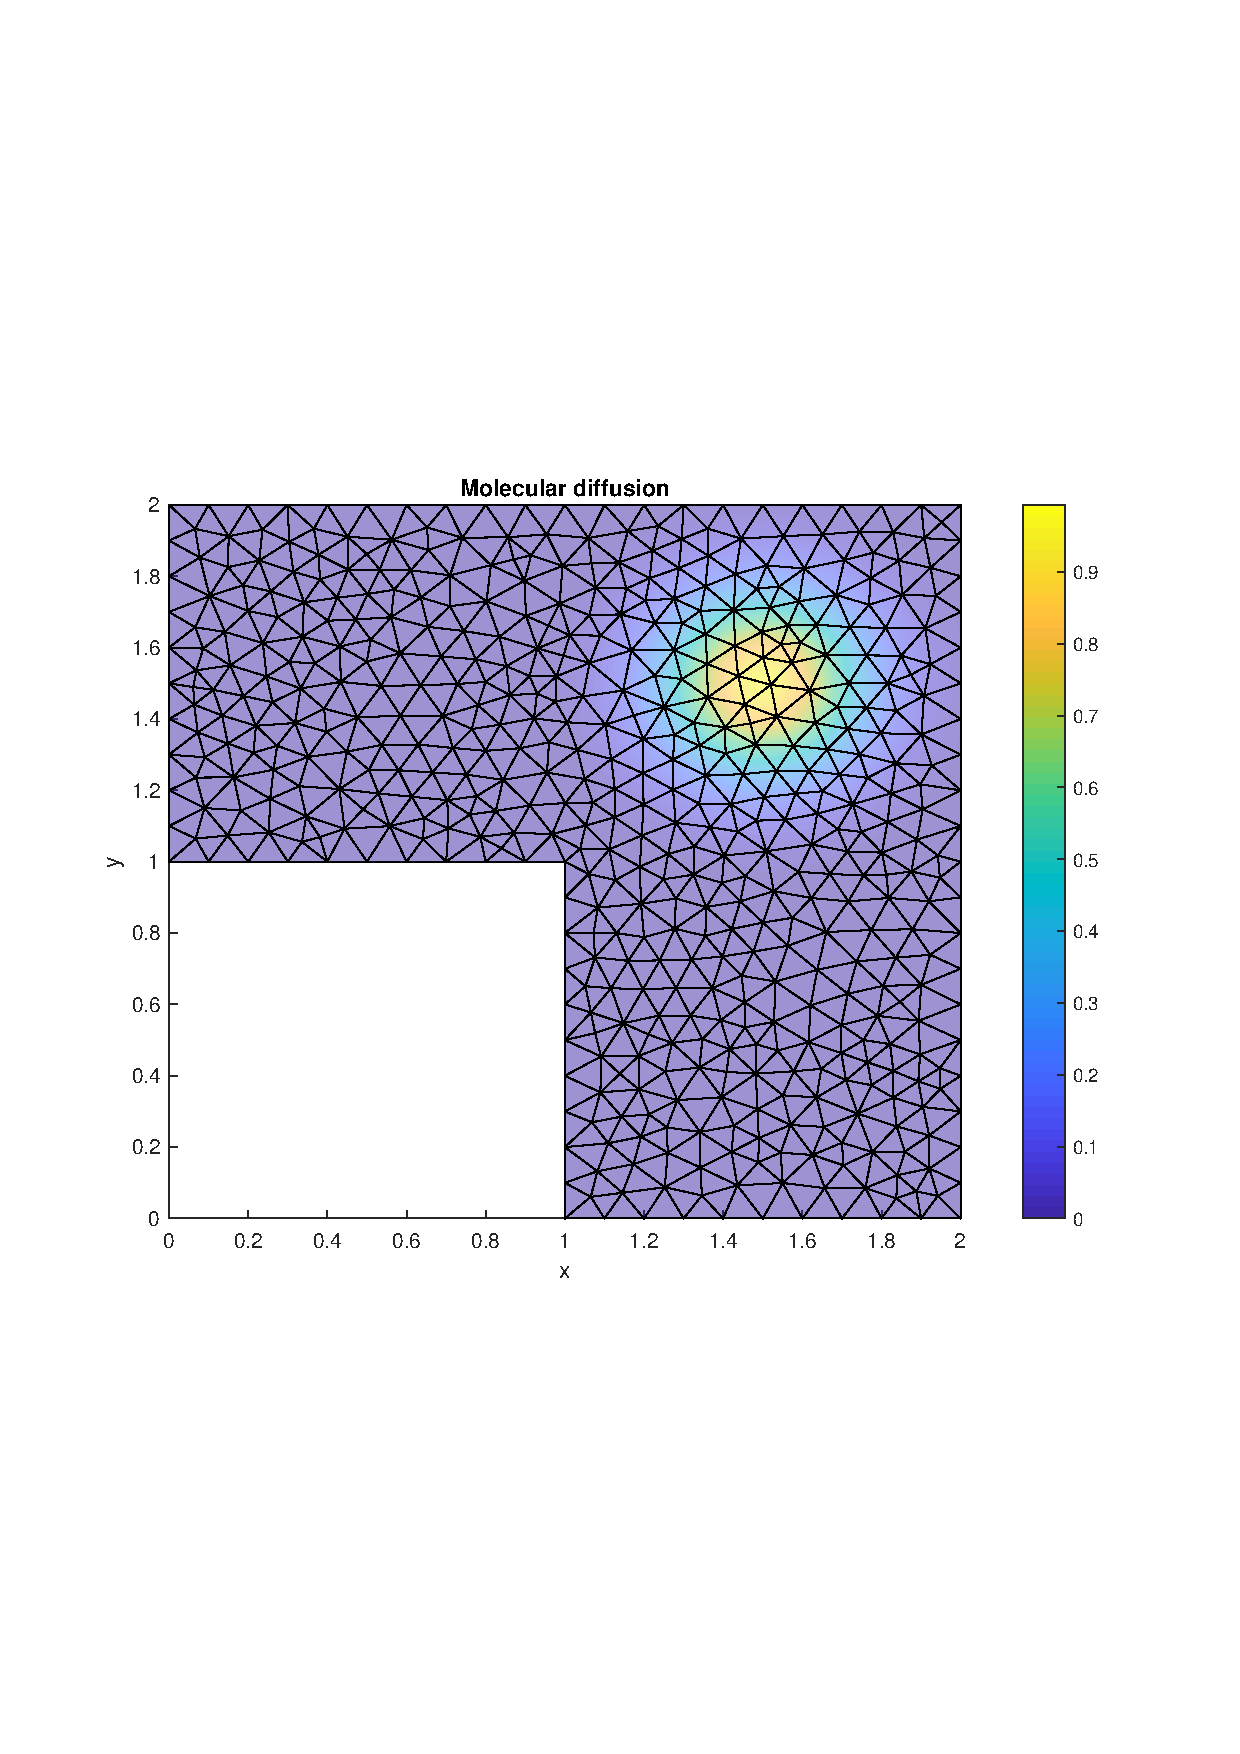
\includegraphics[width=0.49\textwidth]{assets/sol_t0_0090.pdf}
  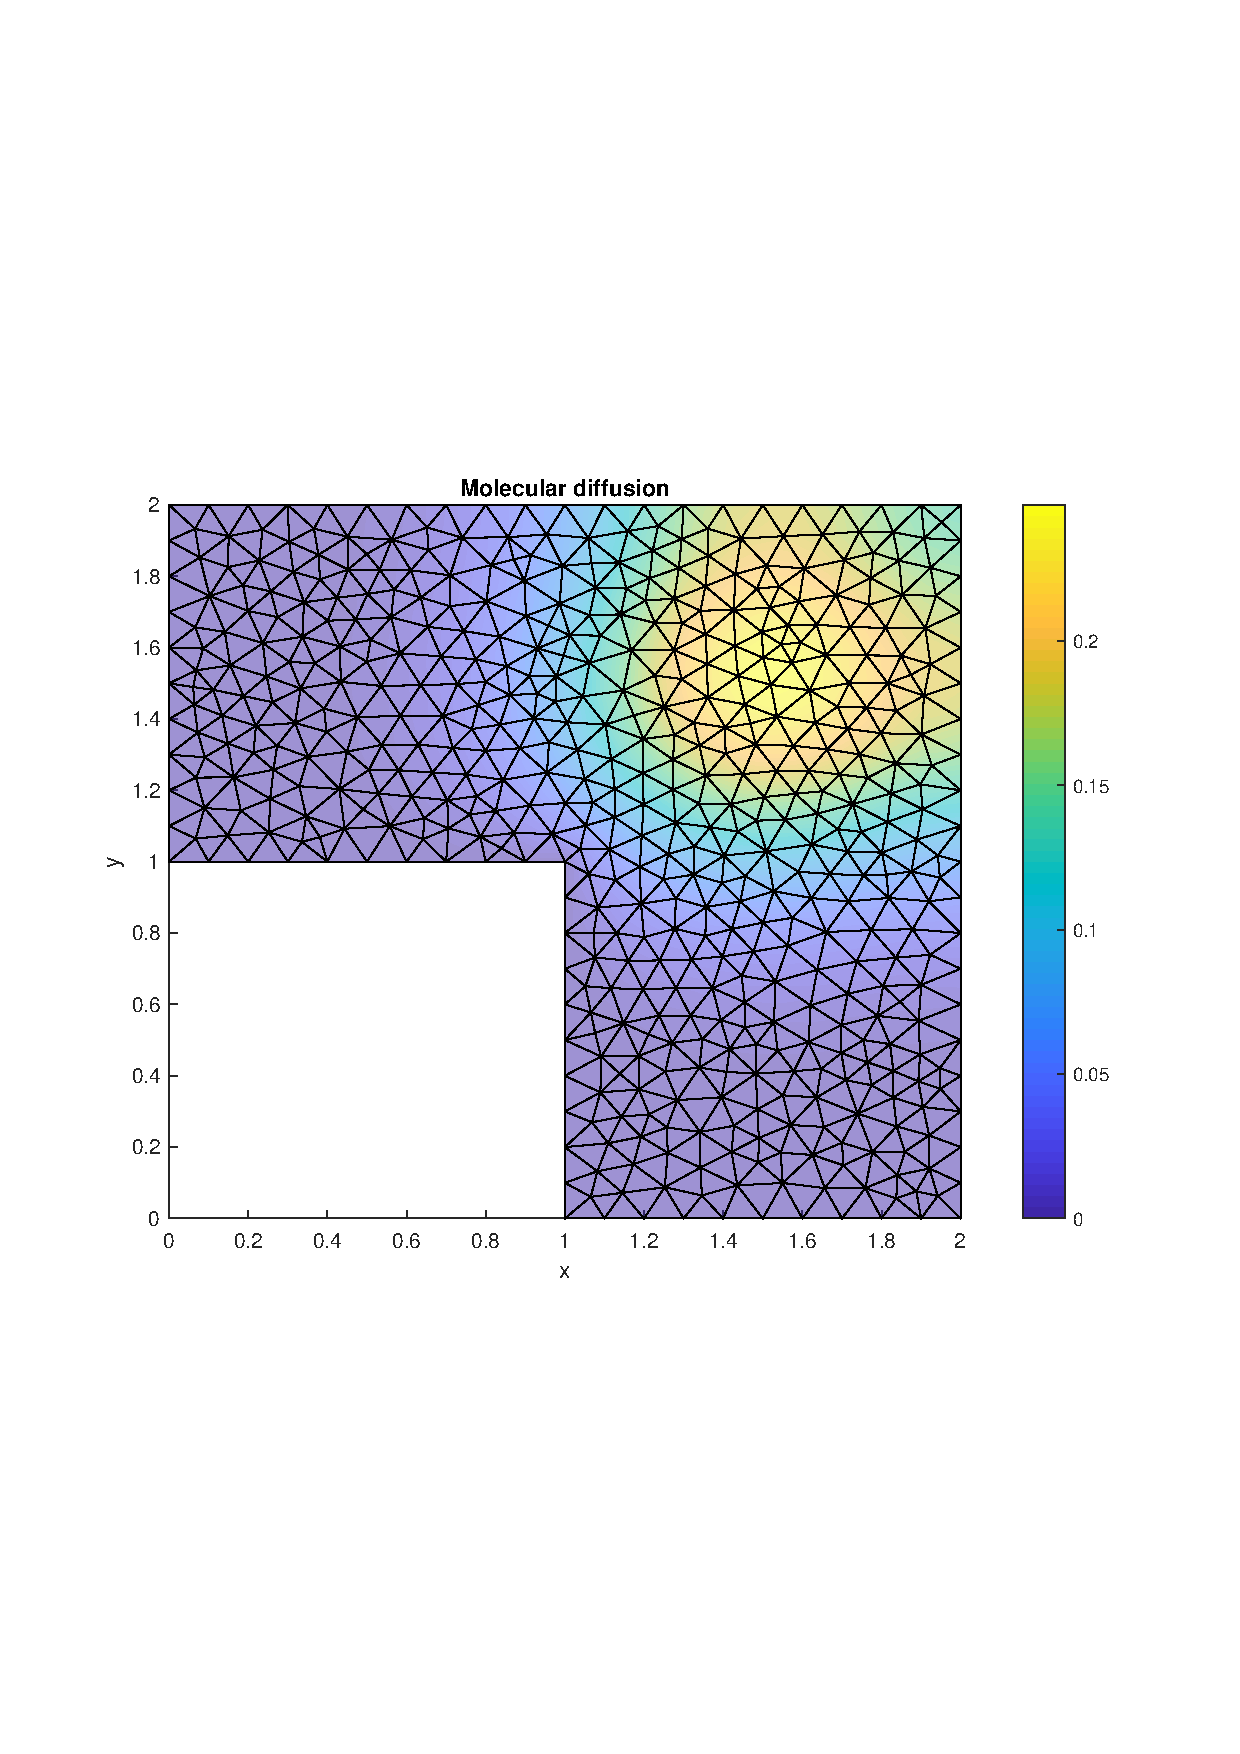
\includegraphics[width=0.49\textwidth]{assets/sol_t1_0090.pdf}
  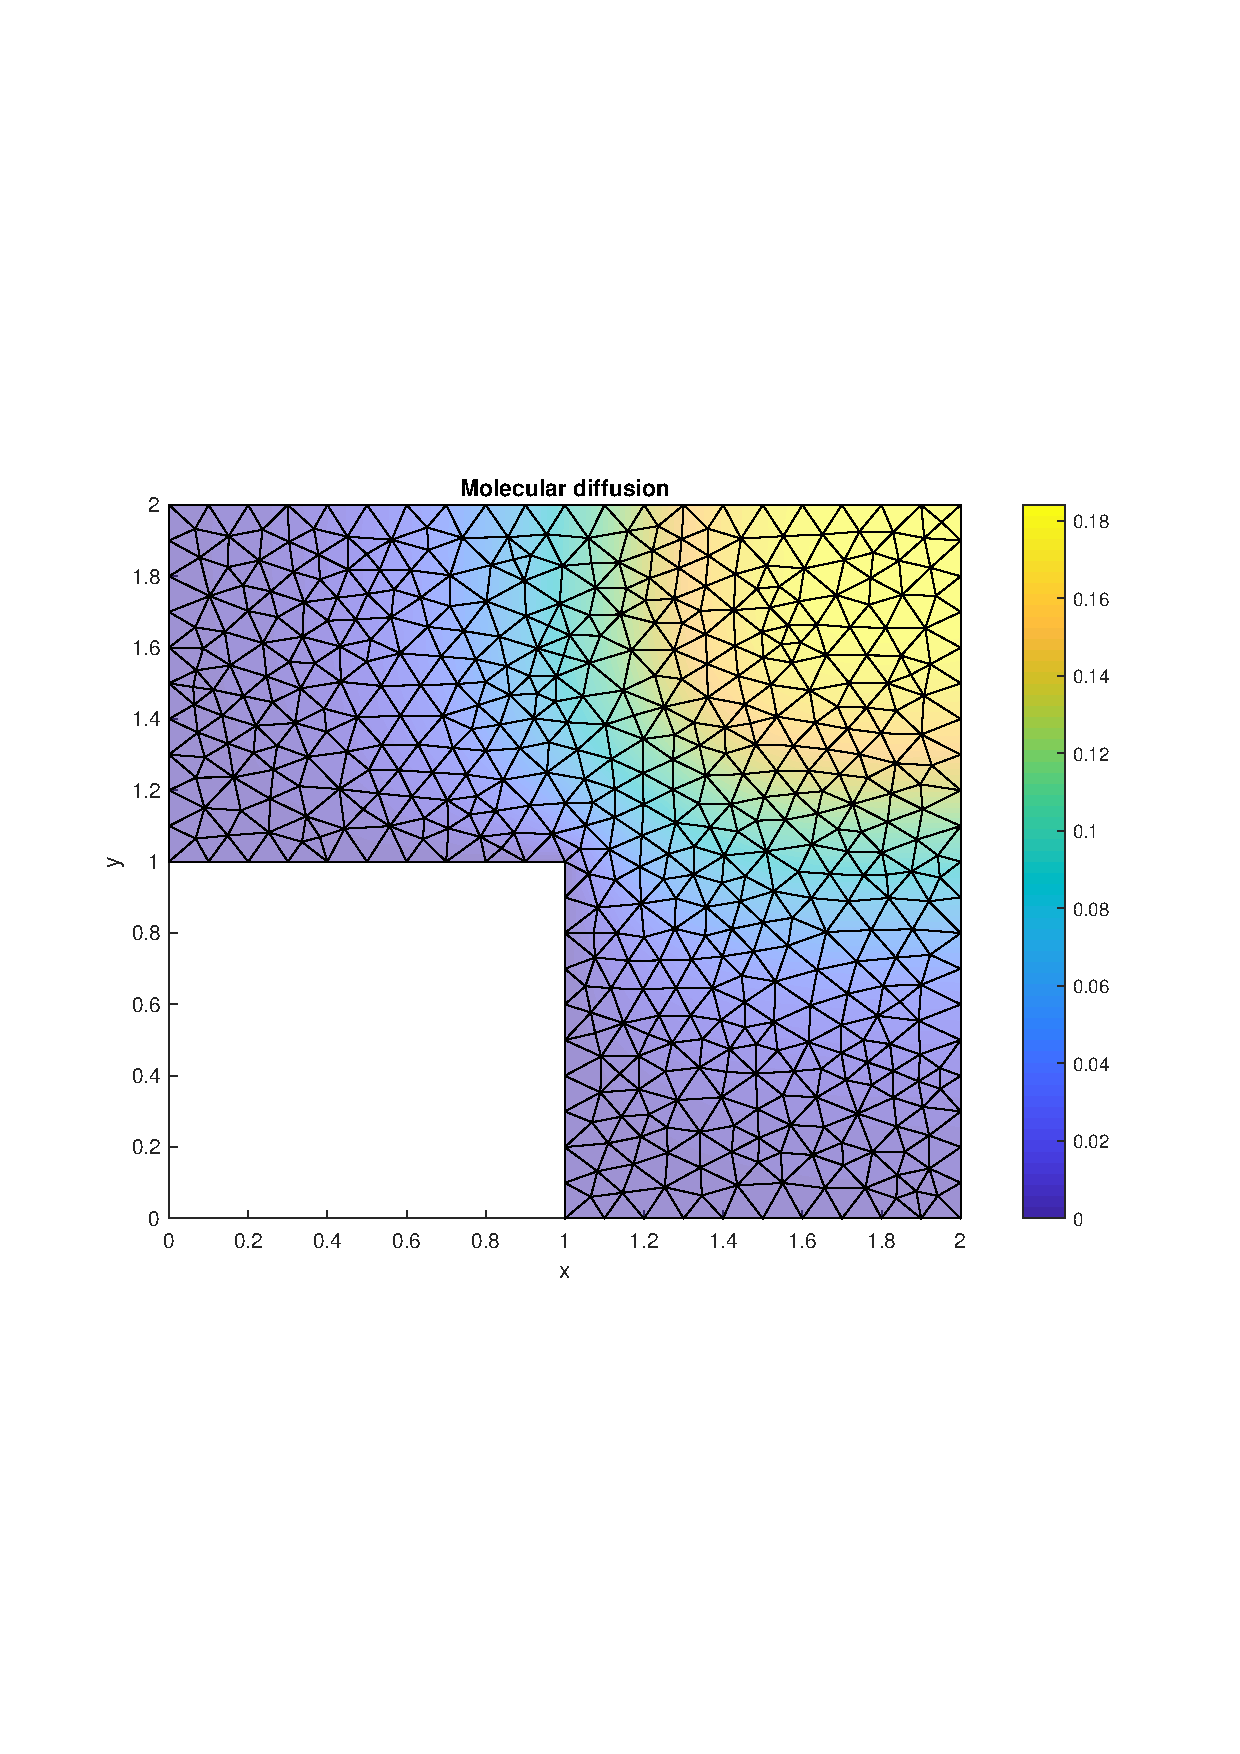
\includegraphics[width=0.49\textwidth]{assets/sol_t2_0090.pdf}
  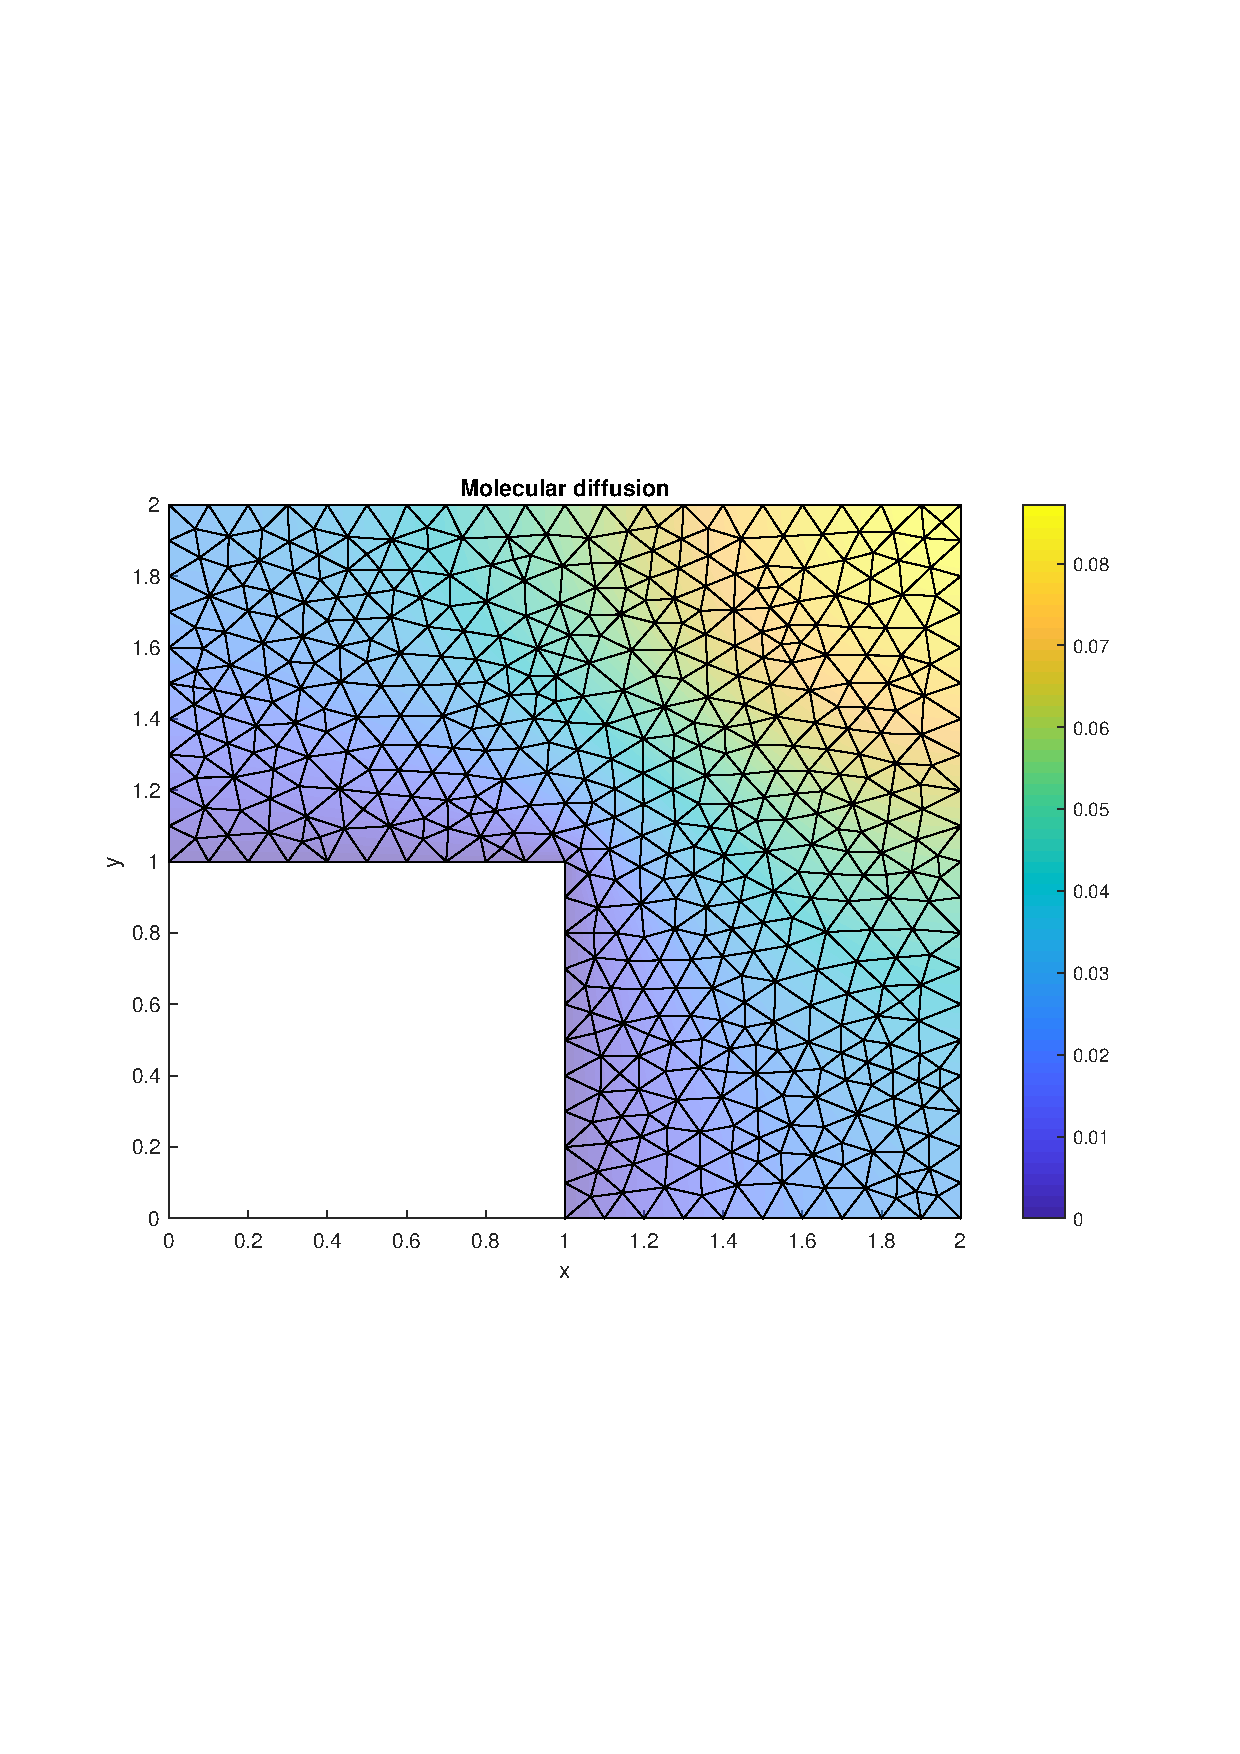
\includegraphics[width=0.49\textwidth]{assets/sol_t10_0090.pdf}
  \caption{Solution $u$ at $t=0$, $t=1$, $t=2$ and $t=10$.}\label{fig:sol90}
\end{figure}
\begin{figure}
  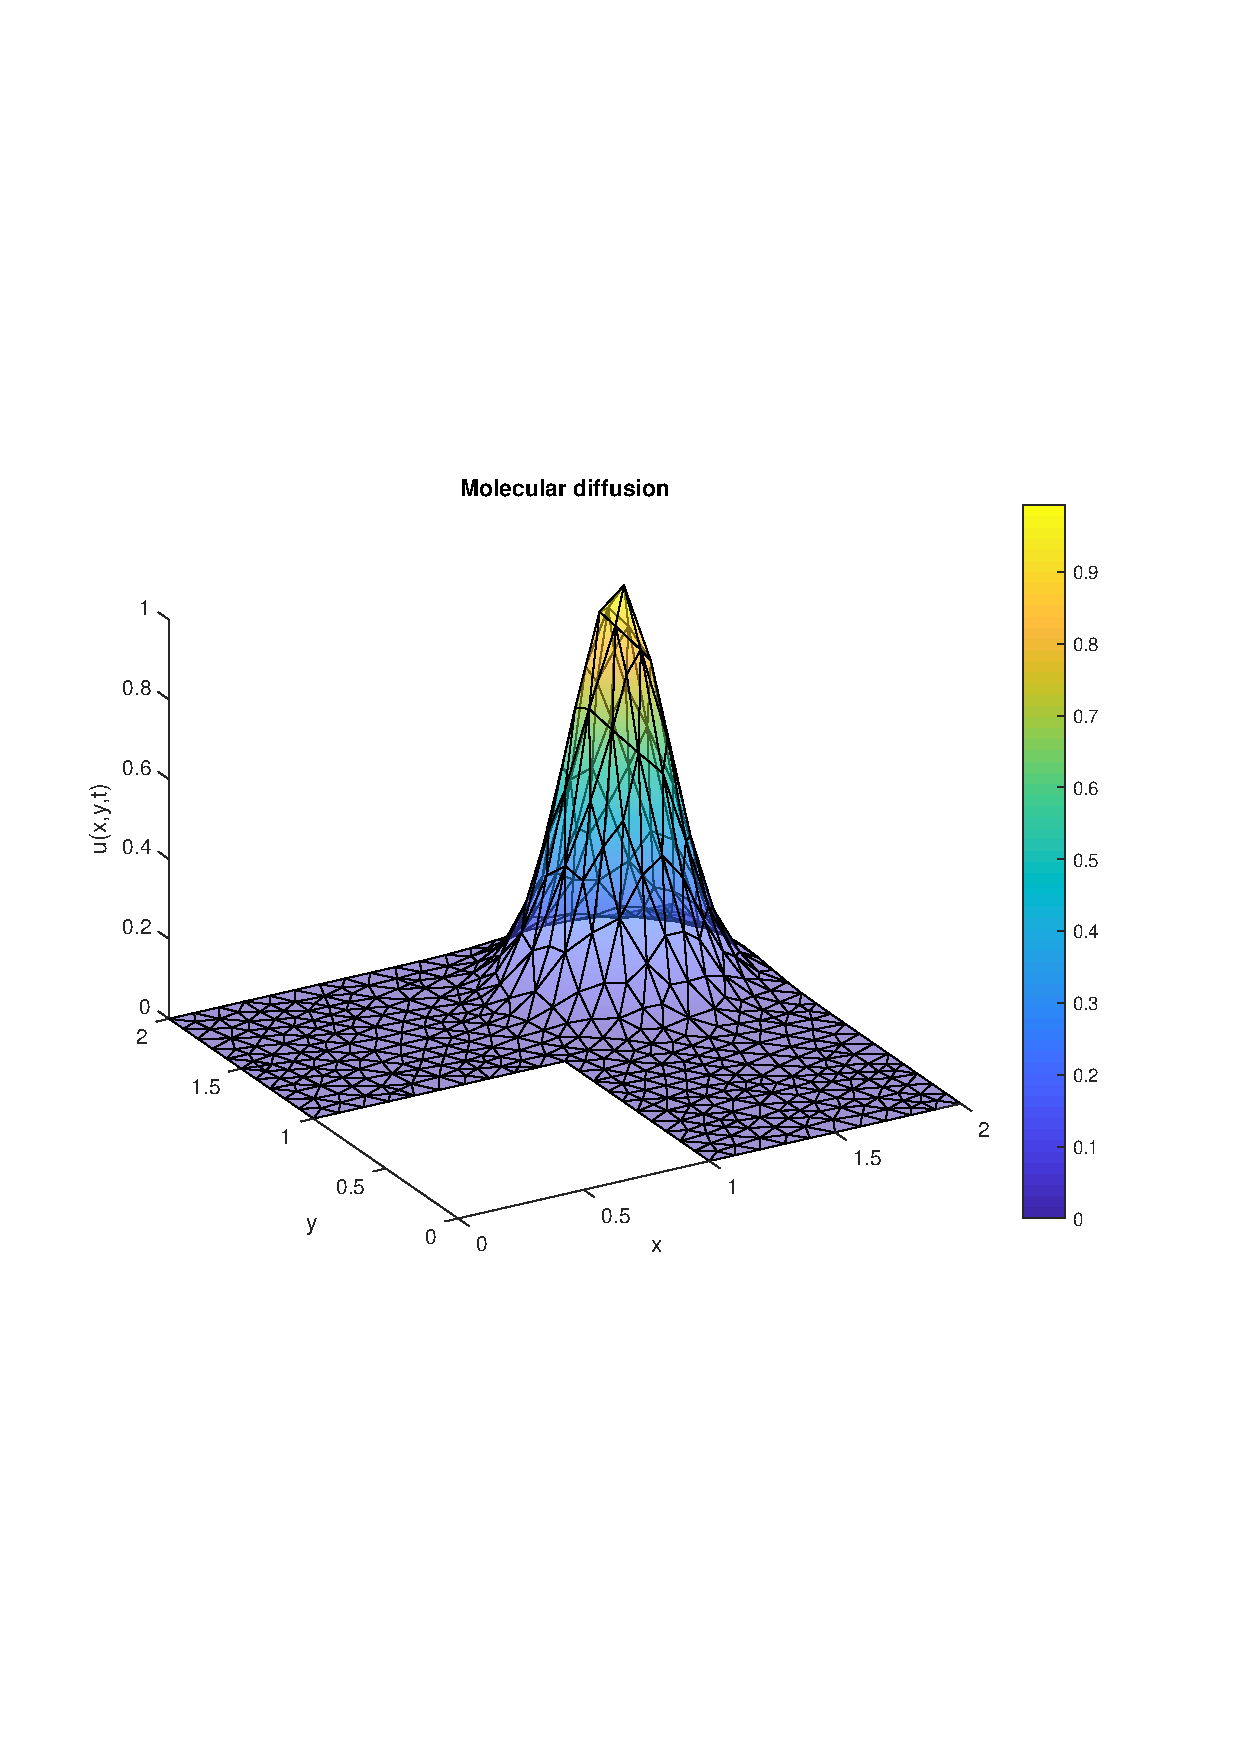
\includegraphics[width=0.49\textwidth]{assets/sol_t0_3030.pdf}
  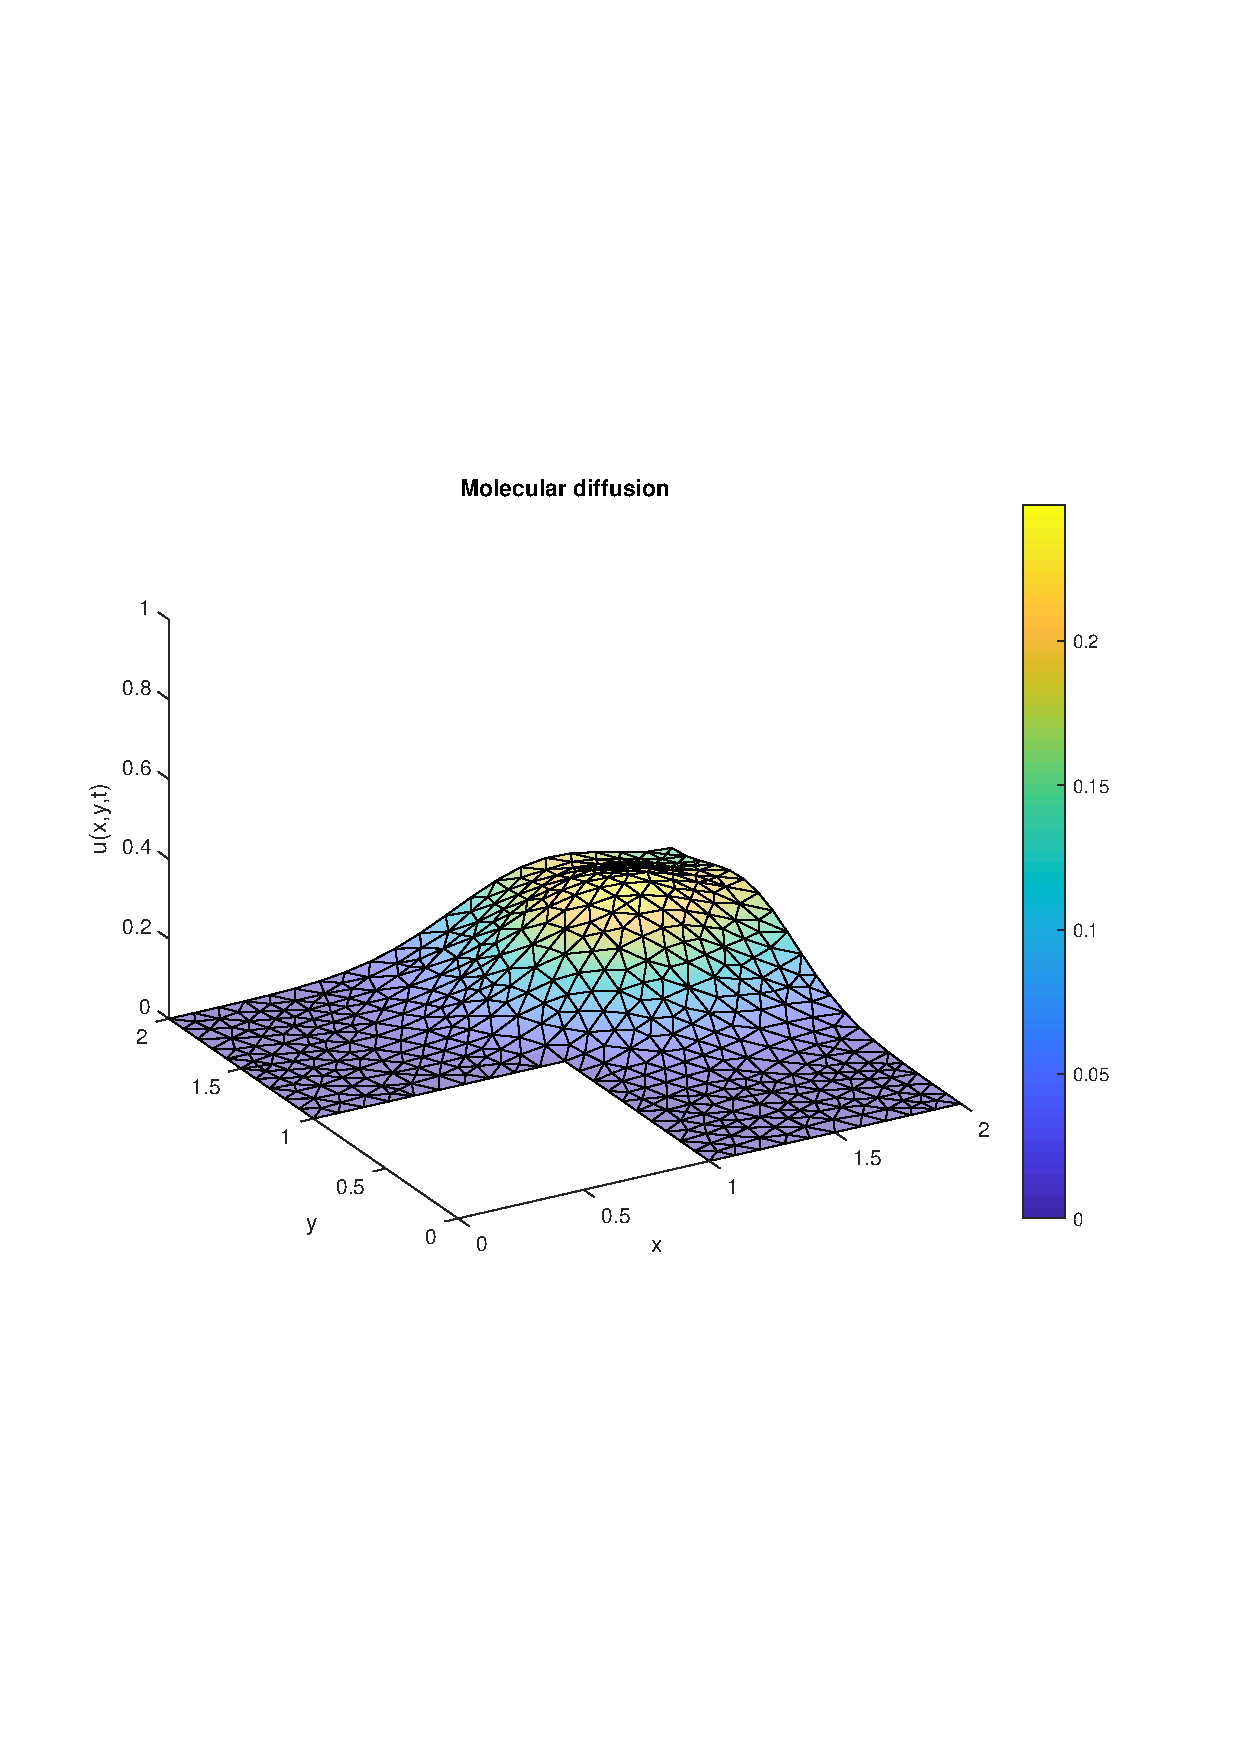
\includegraphics[width=0.49\textwidth]{assets/sol_t1_3030.pdf}
  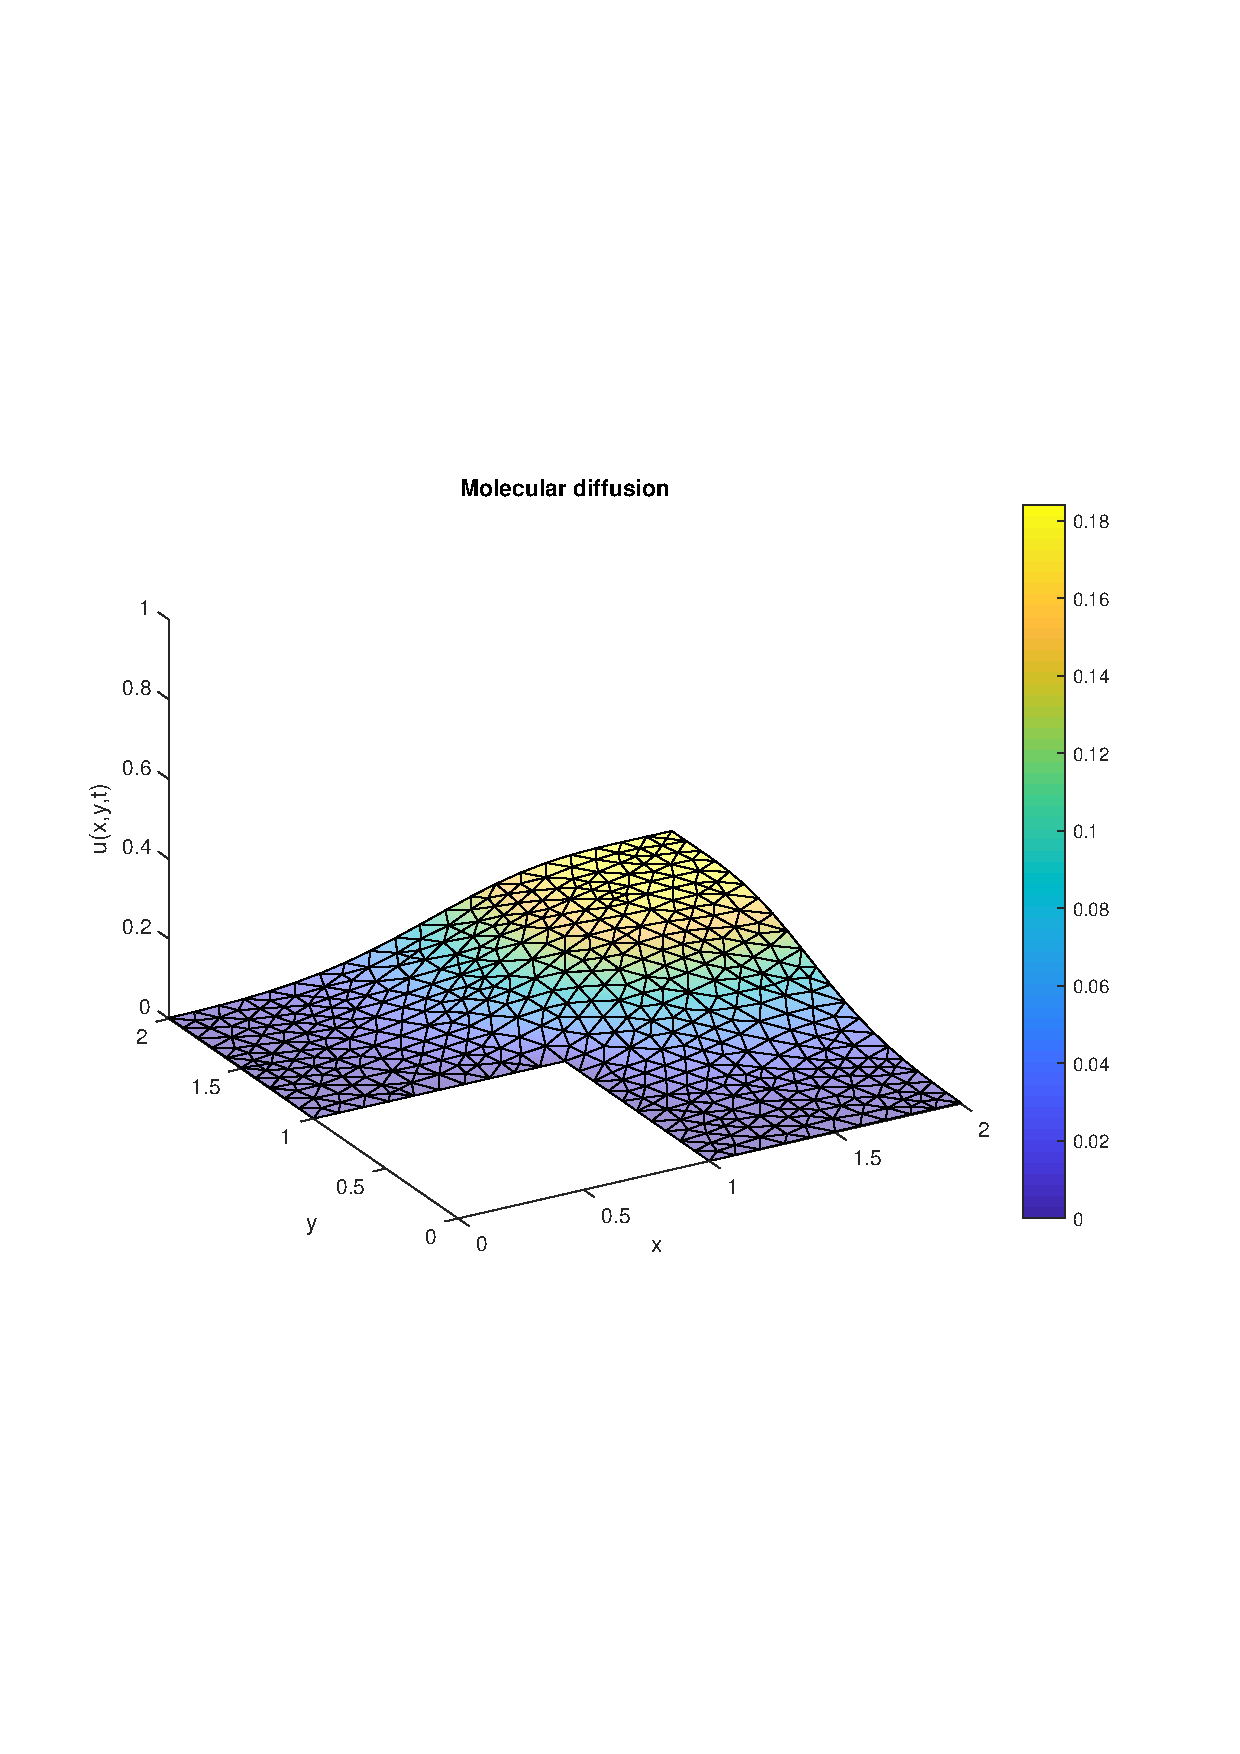
\includegraphics[width=0.49\textwidth]{assets/sol_t2_3030.pdf}
  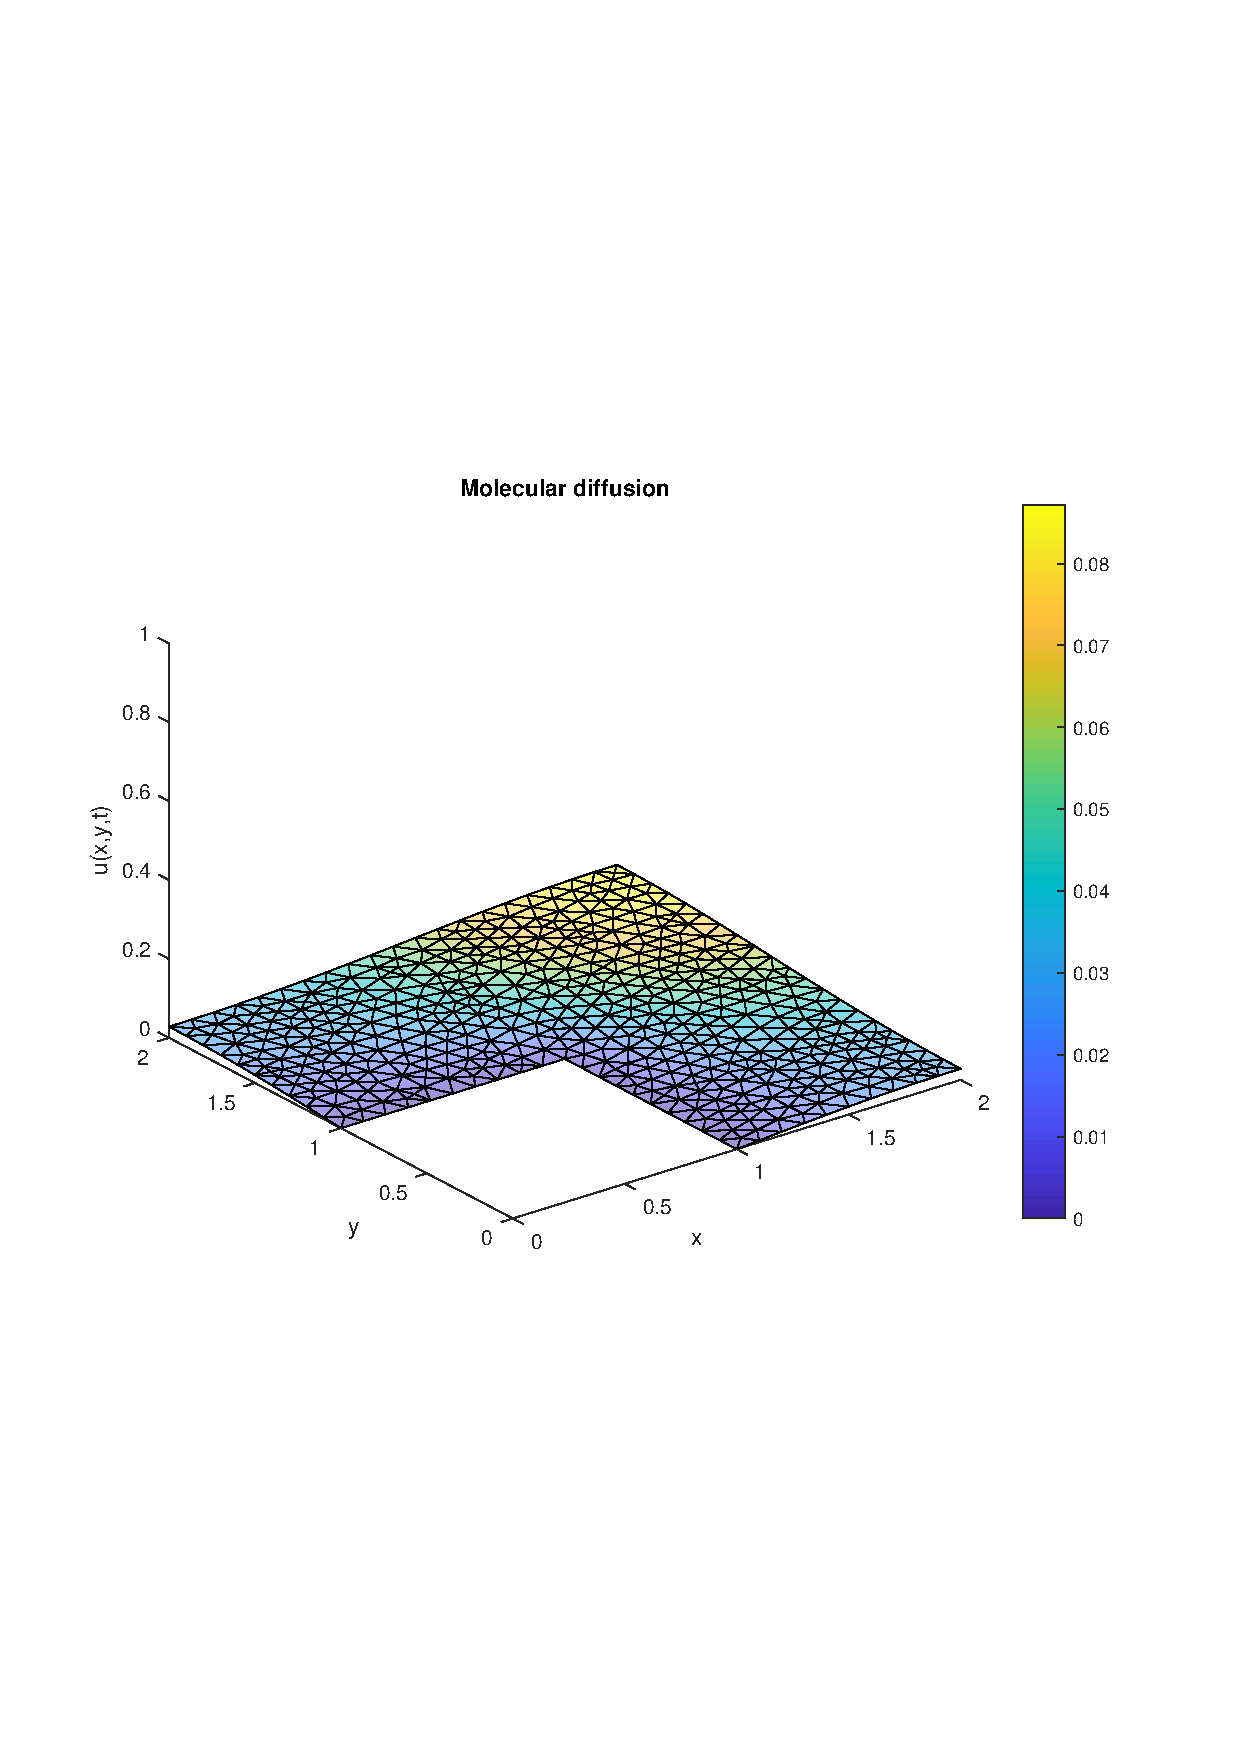
\includegraphics[width=0.49\textwidth]{assets/sol_t10_3030.pdf}
  \caption{Solution $u$ at $t=0$, $t=1$, $t=2$ and $t=10$.}\label{fig:sol90}
\end{figure}
\end{document}
